\documentclass[10pt]{article}
\usepackage[polish]{babel}
\usepackage[utf8]{inputenc}
\usepackage[T1]{fontenc}
\usepackage{amsmath}
\usepackage{amsfonts}
\usepackage{amssymb}
\usepackage[version=4]{mhchem}
\usepackage{stmaryrd}
\usepackage{graphicx}
\usepackage[export]{adjustbox}
\graphicspath{ {./images/} }

\title{GIMNAZJUM }

\author{}
\date{}


\begin{document}
\maketitle
\begin{enumerate}
  \item Rozstrzygnij, czy istnieje taka liczba naturalna \(n\), dla której \(\sqrt[5]{5 n}, \sqrt[6]{6 n}\) i \(\sqrt[7]{7 n}\) są liczbami naturalnymi.
  \item Liczby całkowite \(m\) i \(n\) spełniają równanie
\end{enumerate}

\[
(m-n)^{2}=\frac{4 m n}{m+n-1}
\]

Udowodnij, że liczba \(m+n\) jest kwadratem liczby całkowitej.\\
3. Prostokąt \(A B C D\) podzielono na kwadraty tak, jak na rysunku.

Wiadomo, że \(A B=32 \mathrm{~cm}\). Ile centymetrów długości ma bok \(A D\) ?\\
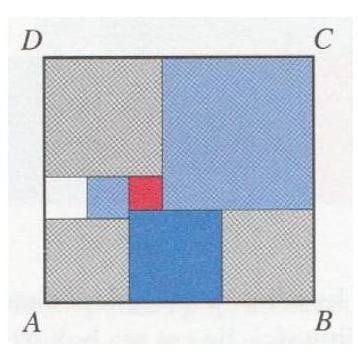
\includegraphics[max width=\textwidth, center]{2024_11_21_6a3dc3e3d38c7fac1bfbg-1(1)}

\section*{LICEUM}
\begin{enumerate}
  \item Rozstrzygnij, czy istnieje taka liczba naturalna \(n\), dla której \(\sqrt[6]{6 n} i \sqrt[8]{8 n}\) są liczbami naturalnymi.
  \item Liczby naturalne \(x\) i \(y\) spełniają warunek \(N W W(x, y)=8 \cdot N W D(x, y)\). Udowodnij, że \(8 x=y\) lub \(8 y=x\).
  \item Na boku \(A B\) równoległoboku \(A B C D\) obrano punkt \(M\), a na bokach AD i CB takie punkty P i Q, że odcinki PM i QM są równoległe do przekątnych równoległoboku. Udowodnij, że trójkąty PDM i QCM mają równe pola.\\
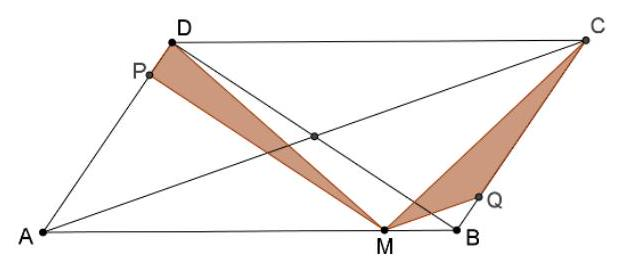
\includegraphics[max width=\textwidth, center]{2024_11_21_6a3dc3e3d38c7fac1bfbg-1}
\end{enumerate}

\end{document}